\providecommand{\isolatedBuild}[1]{#1}% fallback definition lets this file build normally
\isolatedBuild
{
\documentclass[11pt,letterpaper]{book}
\usepackage{import}

% This file must be found via the TEXINPUTS environment variable.
%\documentclass[11pt,letterpaper]{book}

% aleeper: I think these are needed for Paul's macros?
\usepackage{epsfig}
\usepackage{epstopdf}

%\makeatletter
%\typeout{The import path is \import@path}
%\makeatother

\usepackage{import}

\subimport{./}{packagesMitiguy.sty}
\subimport{./}{macrosMitiguy.tex}
\subimport{./}{PageStylesMitiguy.tex}
\subimport{./}{macrosLeeper.tex}


\pagestyle{plain}
\pagenumbering{arabic}

\begin{document}
\HandoutHeader{Vector Equations and Geometry}
%
\vspace{-0.5pc}
\small
%
\begin{enumerate}
\item \textColorBold{darkerBlue}{Cameras and Robotics in the NFL}
\\[0.5pc]
}
%%%%%%%%%%%%%%%%%%%%%%%%%%%%%%%%%%%%%%%%%%%%%%%%%%%%%%%%%%%
%
\begin{minipage}[t]{0.7\linewidth}
The 1st and Ten Graphics System is used to  show a virtual yellow line on video footage of football games.
The system continuously measures the position and orientation of the camera relative to the the field. Hence, position information from the field can be converted into the frame of the camera for overlaying on the video in real-time, even as the camera rotates.
%When an operator clicks on the image, the click location is converted into a position on the field.
\\[0.45pc]
Let the field be a rigid frame \basis{N} with orthogonal unit
vectors \uvecBasisxyz{n} oriented as shown.
Let point $N_o$ be fixed in \basis{N} at zero height above the field.
Assume the field lies in the \uvecxy{n} plane.
%
\\[0.45pc]
Let the camera body be a rigid frame \basis{B} with orthogonal
unit vectors \uvecBasisxyz{b} and a point $B_o$ fixed in \basis{B}.
Assume the position vector from $N_o$ to $B_o$ is known to be $\posvec{N_o}{B_o} = (50\mathrm{~yards})~\uvecx{n} + (20\mathrm{~yards})~\uvecz{n}$.
%
\\[0.45pc] Finally, let the football be identified as point $Q$.

\end{minipage}
\hfill
\begin{minipage}[t]{0.27\linewidth}
\vspace{-0.5pc}
\includegraphics[width=\linewidth]{firstAndTen.jpg}
\end{minipage}
\\[0.2pc]
%
\begin{enumerate}
\item
%\\[0.5pc]
\begin{minipage}[t]{0.6\linewidth}
When the football is lying on the field, the operator clicks on the football in the video.
Assume the click is converted into a direction vector pointing to $Q$ from $B_o$ as $\uvecWithHat{u}^{Q/B_o} = 1~\uvecx{b}$.
\\[0.5pc]
Find a \textbf{system of \boldUnderlineDarkRed{scalar} equations} that can be used to solve for the \underline{\uvecx{n} and \uvecy{n} measures} of the football's position from $N_o$. The rotation table will be formed later; for now you may leave unknown dot-products un-evaluated (such as $\uvecx{b} \cdot \uvecx{n}$).
\\[0.5pc]
To do this, it may help to:
\begin{itemize}
\item Introduce \boldDarkRed{unknown} measures for $Q$'s position from $N_o$ to help you express \posvec{N_o}{Q}.
\item Write \posvec{B_o}{Q} as an \boldDarkRed{unknown} multiple of $\uvecWithHat{u}^{Q/B_o}$.
\item Write a \boldDarkRed{vector loop} equation.
\end{itemize}
\end{minipage}
\hfill
\begin{minipage}[t]{0.35\linewidth}
\flushright
\vspace*{0pt}
\includegraphics[width=\linewidth]{football.png}
\end{minipage}

%%%%%%%%%%%%%%%%%%%%%%%%%%%%%%%%%%%%%%%%%%%%%%%%%
\clearpage
\item
%\hspace*{0pt}%\textbf{( 12 pts )}
%\\[-2.7pc]
\begin{minipage}[t]{0.53\columnwidth}
The camera body is mounted on a pan-tilt mechanism; the ``pan" part lets the camera rotate ``left-and-right" and the ``tilt" part lets the camera rotate ``up-and-down".
\\[1.0pc]
Let the ``pan" portion of the mechanism be a rigid frame \basis{A} with orthogonal unit vectors \uvecxyz{a}. Frame \basis{A} is initially aligned with \basis{N} but is then rotated with $+\uvecz{n}$ sense by an angle $\theta$. (Hint: $\theta$ is the angle between \uvecy{n} and \uvecy{a}.)
\\[1.0pc]
The ``tilt" portion of the mechanism can be assumed to be the same as the camera body frame \basis{B}, which is initially aligned with \basis{A} but is then rotated with $+\uvecy{a}$ sense by an angle $\phi$. (Hint: $\phi$ is the angle between \uvecx{a} and \uvecx{b}.)
\\[1.0pc]
Please \textbf{\underline{write two rotation tables}}: one relating \basis{N} and \basis{A} and one relating \basis{A} and \basis{B}.
\\[0.25pc]
Then \textbf{\underline{explain}} how to obtain the rotation table relating frame \basis{N} and \basis{B} (don't actually compute it).
\end{minipage}
\hfill
\begin{minipage}[t]{0.37\columnwidth}
\flushright
\vspace*{0pt}
\includegraphics[width=7cm]{camera_pan_tilt.jpg}
\end{minipage}

%%%%%%%%%%%%%%%%%%%%%%%%%%%%%%%%%%%%%%%%
\clearpage
\item %\textbf{( 10 pts )}
To save you time, you are given the resulting rotation table relating frame \basis{N} and \basis{B}.
\\[0.5pc]
\rotationTable{n}{b}
{\cos(\theta)\cos(\phi)}{-\sin(\theta)}{\cos(\theta)\sin(\phi)}
{\sin(\theta)\cos(\phi)}{\cos(\theta)}{\sin(\theta)\sin(\phi)}
{-\sin(\phi)}{0}{\cos(\phi)}
\\[1.0pc]
Use your result from part (a) to \textbf{\underline{actually solve for the \uvecx{n} and \uvecy{n} measures}} of the football's position from $N_o$ when $\theta = \degrees{30}$ and $\phi = \degrees{45}$. (I want numbers with appropriate units.)
\vspace{13cm}
%
\item %\textbf{( 5 pts )}
For the actual camera \textit{optical} frame \basis{C}, the convention in the camera industry is to assign orthogonal unit vectors \uvecx{c} to the right, \uvecy{c} down, and \uvecz{c} forward. However, a roboticist created the pan-tilt mechanism and assigned the frames \basis{A} and \basis{B}. From the figure, please \textbf{\underline{write a rotation table}} relating frame \basis{B} and \basis{C}. (There are no angles involved).
\\[1.0pc]
\todo{NEED TO ADD FIGURE}

\end{enumerate}
%
\isolatedBuild { \end{enumerate} \end{document} }
